%q% Based on generic-ornate-15min-45min.en.tex by Till Tantau <tantau@users.sourceforge.net>.
% Ilari Nieminen, 2007. No rights reserved.
% http://www.tcs.hut.fi/Studies/T-79.4001/
% T-79.4001 Seminar on Theoretical Computer Science

% Original copyright notice:

% http://www.lirmm.fr/~fiorio/AlgorithmSty/ (Place algorithm2e.sty in your working directory)

\documentclass[12pt]{beamer} 
\usepackage{times}
\usepackage[]{algorithm2e}
%\SetKw{def}{def}
%\SetKw{To}{to} 
%\SetKw{Othera}{other}
%\SetKw{Become}{become}

\usepackage[T1]{fontenc} % bedre orddeling og ofte påkrævet at
\usepackage[utf8]{inputenc} % eller utf8 eller ansinew eller ...
\usepackage[english, danish]{babel} %direktiv til at bruge det danske sprog

\renewcommand\danishhyphenmins{22} % bedre orddeling
\addto\captionsdanish{
\renewcommand\contentsname{Indholdsfortegnelse}
\renewcommand\appendixname{Appendix}
}
\selectlanguage{danish}
 
\usepackage[]{booktabs}
\usepackage{listings}
 \lstset{ 
         basicstyle=\tiny\ttfamily, % Standardschrift
         numbers=left,               % Ort der Zeilennummern
         numberstyle=\tiny,          % Stil der Zeilennummern
         stepnumber=2,               % Abstand zwischen den Zeilennummern
         numbersep=5pt,              % Abstand der Nummern zum Text
         tabsize=2,                  % Groesse von Tabs
         extendedchars=true,         %
         breaklines=false,            % Zeilen werden Umgebrochen
         keywordstyle=\color{red},
                frame=b,         
         keywordstyle=[1]\textbf,    % Stil der Keywords
         keywordstyle=[2]\textbf,    %
         keywordstyle=[3]\textbf,    %
         keywordstyle=[4]\textbf,   %\sqrt{\sqrt{}} %
         stringstyle=\color{black}\ttfamily, % Farbe der String
         showspaces=false,           % Leerzeichen anzeigen ?
         showtabs=false,             % Tabs anzeigen ?
         xleftmargin=17pt,
         framexleftmargin=17pt,
         framexrightmargin=5pt,
         framexbottommargin=4pt,
         %backgroundcolor=\color{lightgray},
         showstringspaces=false      % Leerzeichen in Strings anzeigen ?        
 }

 \lstloadlanguages{% Check Dokumentation for further languages ...
         [Visual]Basic,
         Pascal,
         C,
         C++,
         XML,
         HTML,
         PYTHON,
 }
\lstset{language=Python}
\lstset{emph={@process, @choise,choice, Alternation, Skip,Timeout,Parallel,Sequence, Spawn,@io,ChannelPoisonException, ChannelRetireException},emphstyle=\underbar}

\newcommand\mc[1]{\multicolumn{1}{c}{\textbf {#1}}} % sparer plads


% A few keywords to use in pseudocode
% You should also probably read the algorithm2e -documentation more than I did.

\usetheme[nat,dk,style=simple]{Frederiksberg}% Beamer theme v 3.0
%\mode<presentation>
%{
%\usetheme{Rochester}% Beamer theme v 3.0
%\usecolortheme{whale}
%   \setbeamercovered{transparent}
%   \definecolor{beamer@tkkblue}{HTML}{0041AD}
%   \setbeamercolor{structure}{fg=beamer@tkkblue}
%} 
\title
{Timed PyCSP}
%\subtitle
%{Specialeforsvar}
\institute
{Datalogisk Institut \\ Københavns Universitet}
\author
{Rasmus Ebdrup Sørensen}
\date
{5. juli 2010}


\begin{document}

\frame[plain]\titlepage

\begin{frame}
  \frametitle{Oversigt}
  \tableofcontents
\end{frame}

\section{Motivation og mål}
%\subsection{Motivation}
\begin{frame}
  \frametitle{Tid}
  \begin{itemize}
	\item Fundamental egenskab
	\item Global
	\item Relevant ved interaktion med, eller simulering af virkeligheden
	\item - Eksempelvis vejrsystemer, trafik, kontrolsystemer 
  \end{itemize}
\end{frame}

\begin{frame}
  \frametitle{CSP}
  \begin{itemize}
	\item  Nem repræsentaion af samtidighed
	\item Eksplicit udveksling af data
	\item Ingen delte datastrukturer
 \end{itemize}
\end{frame}

%\subsection{Mål}
\begin{frame}
  \frametitle{Introduktion af tid i CSP}
  \begin{itemize}
	\item Tilbyde en ensartet håndtering af tid i CSP
	\item Let at anvende
	\item Brugbar
	\item håndtere tilstande tilknyttet tid, som ikke direkte er relateret til problemet
  \end{itemize}
\end{frame}

\section{PyCSP}
%\subsection{Kort overblik}
\begin{frame}		
  \frametitle{PyCSP}
  \begin{itemize}
  \item Skrevet i Python
	\item Greenlets-versionen pga. scheduler
	\item Greenlets er små bruger-tråde
	\item hurtige processkift, samt oprettelse og nedlæggelse af dem
	\item Kun Any-to-Any kanaler
  \end{itemize}
\end{frame}

\section{Tidsmodeller}
\begin{frame}
	\frametitle{Tre avendelsesområder}
	\begin{itemize}
		\item Diskret event simulering (DES)
		\item Realtids planlægning (RTP)
		\item interaktiv planlægning (IP)
	\end{itemize}
\end{frame}

\begin{frame}
	\frametitle{To tidsmodeller}
	\begin{itemize}
		\item Diskret tid
		\begin{itemize}
			\item Drives af begivenheder
			\item variable tidsskridt
			\item Har et starttidspunkt
 		\end{itemize}
		\item Real tid
		\begin{itemize}
			\item Drives af tiden selv
			\item Faste tidsskridt
			\item Kan have et starttidspunkt
			\item Kan have en deadline.
		\end{itemize}
	\end{itemize}
\end{frame}

\section{DES}

\begin{frame}
  \frametitle{DES Eksempel}
\begin{figure}
 \begin{center}
  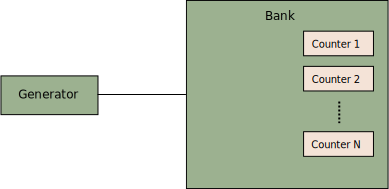
\includegraphics[scale=0.75]{bank_example}
	\caption{Kunder i en bank}
	\label{fig:hard-rtp}
\end{center}
\end{figure}
\end{frame}

\begin{frame}
  \frametitle{Krav til DES}
  \begin{itemize}   
	\item Repræsentation af tid
	\item Liste af begivenheder
	\item Opsamling af statistisk data
  \end{itemize}
  \begin {itemize}
  \item Kan håndteres uden Timed PyCSP \\
   - Vi gør det bare bedre
  \end{itemize}
\end{frame}

\begin{frame}
\frametitle{Implementering}
  \begin{itemize}   
	\item Now()
	\item Wait()
	\item Plotter
	\item Udvide scheduler
  \end{itemize}
\end{frame}

%\subsection{Resultater}
\begin{frame}[fragile]
  \frametitle{Greenlets-version}
\begin{lstlisting}
@process
def Generator(i,number,meanTBA, meanWT,
              customerWRITER,barrierWRITER,barrierREADER):
  t_event = 0
  time = 0
  numberInserted = 0
  while numberInserted<number:
    if t_event<=time:
      customerWRITER(Customer(name = "Customer%d:%02d"%
                     (i,numberInserted),meanWT=meanWT))
      t_event = time + round(expovariate(1/meanTBA))
      numberInserted+=1
    barrierWRITER(0)
    barrierREADER()
    time+=1
  retire(customerWRITER)
  try:
    while True:
      barrierWRITER(0)
      barrierREADER()
      time +=1
  except ChannelPoisonException: 
    return
\end{lstlisting}
\end{frame}

\begin{frame}[fragile]
  \frametitle{DES-version}
\begin{lstlisting}
@process
def Generator(i,number,meanTBA, meanWT, customerWRITER):
  for numberInserted in range(number):
    customerWRITER(Customer(name = "Customer%d:%02d"%(i,numberInserted),
                            meanWT = meanWT))
    Wait(expovariate(1/meanTBA))
  retire(customerWRITER)
\end{lstlisting}
\end{frame}

\section{RTP}

\begin{frame}
  \frametitle{RTP Eksempel}
  \begin{figure}
 \begin{center}
  
\includegraphics[scale=0.75]{pig-network}
	\caption{Udskæring af grise på et slagteri}
	\label{fig:hard-rtp}
\end{center}
\end{figure}

\end{frame}

%Typer af deadline og Hard real time
\begin{frame}
  \frametitle{Krav til RTP}
  \begin{itemize}   
	\item Processer skal have en  deadline
	\item Scheduleringsalgoritme, EDF
	\item DeadlineException
  \end{itemize}
\end{frame}

%Wait i RTP
\begin{frame}
  \frametitle{Implementering}
  \begin{itemize}   
    \item Set\_deadline() og Remove\_deadline()
    \item Set\_priority() og Remove\_priority()
    %\item Deadline exception
    \item Now()
    \item Wait()
    \item Scheduler 
	%\begin{itemize}
	%	\item has$\_$priority 
	%	\item no$\_$priority
	%	\item timers
	%\end{itemize}
	\item Prioritetsinvertering
	\item Prioritetsnedarvning
  \end{itemize}
\end{frame}


%\begin{frame}
%\frametitle{Kommunikation}
%\begin{itemize}
%	\item Udfordring ved Any-to-Any Kanaler 
% 	\item Alternation
%\end{itemize} 
%\end{frame} 

%\subsection{Resultater}


\begin{frame}
  	\frametitle{RTP resultater}
	\tiny 
	\begin{table}[htbp]
		\centering
		\begin{tabular}{lcccc}
		   	\toprule
		    \mc{Version}&\mc{Tid i dummyproces(s)}&\mc{SA.}& \mc{Succesrate (\%)}&\mc{SA.}\\
		    \midrule
		    Greenlets         & 1.29 & 0.61 & 13 & 2  \\
		    RTP u. prioritet  & 1.05 & 0.28 & 24 & 6  \\
		    RTP m. prioritet  & 0.74 & 0.34 & 42 & 13 \\
		    \bottomrule
		\end{tabular}
		\caption[]{\tiny 10 * 100 grise køres igennem procesnetværket. Samtidigt køres en dummyproces.}
	\end{table}
\end{frame}

\begin{frame}
\frametitle{RTP resultater}
\tiny 
\begin{table}[htbp]
	\centering
	\begin{tabular}{lccc}
       	\toprule
        \mc{Version}  &\mc{Samtidige grise} & \mc{Succesrate (\%)} & \mc{Standard Afvigelse (SA)} \\
%       \midrule
%      Processes        & 1 & 16 & 2 \\
%       Processes        & 2 &  0 & 0 \\
%       Processes        & 3 &  0 & 0 \\
%       Processes        & 5 &  0 & 0\\
%       \midrule
%       Threads          & 1 & 34 & 6 \\
%       Threads          & 2 &  1 & 1 \\
%       Threads          & 3 &  1 & 0 \\
%       Threads          & 5 &  1 & 1 \\
        \midrule
        Greenlets        & 1 & 44 & 7 \\
        Greenlets        & 2 & 49 & 1 \\
        Greenlets        & 3 & 32 & 0\\
        Greenlets        & 5 & 20 & 0 \\
        \midrule
        RTP u. prioritet & 1 & 42 & 6 \\
        RTP u. prioritet & 2 & 44 & 2 \\
        RTP u. prioritet & 3 & 31 & 2 \\
        RTP u. prioritet & 5 & 19 & 0 \\
        \midrule
        RTP m. prioritet & 1 & 44 & 10\\
        RTP m. prioritet & 2 & 21 & 5\\
        RTP m. prioritet & 3 & 21 & 7\\
        RTP m. prioritet & 5 &  7 & 3\\
 
        \bottomrule
    \end{tabular}
	\caption[]{\tiny 10 kørsler hvor 100 grise bliver sendt igennem procesnetværket. }
\end{table}
\end{frame}

\section{Fremtidigt arbejde}
\begin{frame}
  	\frametitle{Fremtidigt arbejde}
\begin{itemize}
\item DES
	\begin{itemize}
	\item Dynamisk køskifte
	\item Reservering af flere ressurcer
	\item Stopkriterium
	\item Parallelisering
	\end{itemize}
\item RTP
	\begin{itemize}
	\item Estimater for udførselstid
	\item Samarbejde med operativsystemet
	\item Forskellige typer deadlines
	\end{itemize}
\end{itemize}
\end{frame}


%    \item Barrierer
%	\item shared memory
%    \item Sætte begrænsning på kommunikation ifh. til tid.


%\begin{frame}
%  \frametitle{Anvendelse}
%  \begin{itemize}
%	\item MIG
%	\item GRISE
%	\item Fabrik
%	\item Trafik
%	\item vejr, hav forudsigelser mv,
%  \end{itemize}
%\end{frame}


%\begin{frame}
%  \frametitle{TID}
%  \begin{itemize}
%	\item Forventet mål 3-5 min
%	\item Tidsmodel
%	\item DES 10 min.
%	\item RTP 5 min.
%	\item Finale 5 min.
%  \end{itemize}
%\end{frame}

\end{document}

 
